
%(BEGIN_QUESTION)
% Copyright 2010, Tony R. Kuphaldt, released under the Creative Commons Attribution License (v 1.0)
% This means you may do almost anything with this work of mine, so long as you give me proper credit

The flow computer connected to this turbine flowmeter (with electronic pick-up) does not register any flow, even though we know there to be fluid flowing through the pipe.  A voltmeter connected between terminals TB1-1 and TB1-3 registers approximately 11.0 volts DC, and 10.8 volts AC at a frequency of 86 Hz:

$$\includegraphics[width=15.5cm]{i00500x01.eps}$$

Determine the diagnostic value of each of the following tests.  Assume only one fault in the system, including any single component or any single wire/cable/tube connecting components together.  If a proposed test could provide new information to help you identify the location and/or nature of the one fault, mark ``yes.''  Otherwise, if a proposed test would not reveal anything relevant to identifying the fault (already discernible from the measurements and symptoms given so far), mark ``no.''

% No blank lines allowed between lines of an \halign structure!
% I use comments (%) instead, so that TeX doesn't choke.

$$\vbox{\offinterlineskip
\halign{\strut
\vrule \quad\hfil # \ \hfil & 
\vrule \quad\hfil # \ \hfil & 
\vrule \quad\hfil # \ \hfil \vrule \cr
\noalign{\hrule}
%
% First row
{\bf Diagnostic test} & {\bf Yes} & {\bf No} \cr
%
\noalign{\hrule}
%
% Another row
Measure DC voltage between terminals TB2-5 and TB2-8 &  &  \cr
%
\noalign{\hrule}
%
% Another row
Measure resistance between TB2-7 and TB2-8 with the 1 amp fuse pulled &  &  \cr
%
\noalign{\hrule}
%
% Another row
Measure DC voltage across 100 mA fuse &  &  \cr
%
\noalign{\hrule}
%
% Another row
Measure DC voltage across 1 amp fuse &  &  \cr
%
\noalign{\hrule}
%
% Another row
Measure AC voltage between terminals TB3-9 and TB3-11 &  &  \cr
%
\noalign{\hrule}
%
% Another row
Measure continuity of conductor connecting terminals TB1-4 and TB2-8 &  &  \cr
%
\noalign{\hrule}
} % End of \halign 
}$$ % End of \vbox

\vfil 

\underbar{file i00500}
\eject
%(END_QUESTION)





%(BEGIN_ANSWER)

This is a graded question -- no answers or hints given!

%(END_ANSWER)






%(BEGIN_NOTES)

The presence of both DC and AC voltage at the flowmeter's pulse output tells us we have good continuity between the 24 VDC source and the transmitter, and also that the switching transistor is indeed pulsing on and off.  If it were on continuously, we would measure only a few tenths of a volt DC.  If it were off continuously, we would measure a full 24 VDC all the time.

An AC voltage registered by our voltmeter tells us it is seeing an {\it oscillating} voltage over time.  This tells us the transistor is indeed switching on and off as it should.  In this state of sensing a square-wave signal, the voltmeter will register a DC voltage that is approximately one-half of the DC source voltage because it is averaging the high and low voltage values of the square wave signal.  With a 50\% duty cycle, the average DC voltage will be 50\% of the DC source voltage.

\vskip 10pt

The problem, therefore, is either in the optocoupler or past it (toward the flow computer).  Any test performed to check wiring on the flowmeter's circuit (aside from perhaps checking the diode in the optocoupler) is therefore a wasted test.

% No blank lines allowed between lines of an \halign structure!
% I use comments (%) instead, so that TeX doesn't choke.

$$\vbox{\offinterlineskip
\halign{\strut
\vrule \quad\hfil # \ \hfil & 
\vrule \quad\hfil # \ \hfil & 
\vrule \quad\hfil # \ \hfil \vrule \cr
\noalign{\hrule}
%
% First row
{\bf Diagnostic test} & {\bf Yes} & {\bf No} \cr
%
\noalign{\hrule}
%
% Another row
Measure DC voltage between terminals TB2-5 and TB2-8 &  & $\surd$ \cr
%
\noalign{\hrule}
%
% Another row
Measure resistance between TB2-7 and TB2-8 with the 1 amp fuse pulled &  & $\surd$ \cr
%
\noalign{\hrule}
%
% Another row
Measure DC voltage across 100 mA fuse & $\surd$ &  \cr
%
\noalign{\hrule}
%
% Another row
Measure DC voltage across 1 amp fuse &  & $\surd$ \cr
%
\noalign{\hrule}
%
% Another row
Measure AC voltage between terminals TB3-9 and TB3-11 & $\surd$ &  \cr
%
\noalign{\hrule}
%
% Another row
Measure continuity of conductor connecting terminals TB1-4 and TB2-8 &  & $\surd$ \cr
%
\noalign{\hrule}
} % End of \halign 
}$$ % End of \vbox

\vfil \eject

\vskip 20pt \vbox{\hrule \hbox{\strut \vrule{} {\bf Virtual Troubleshooting} \vrule} \hrule}

This question is a good candidate for a ``Virtual Troubleshooting'' exercise.  Presenting the diagram to students, you first imagine in your own mind a particular fault in the system.  Then, you present one or more symptoms of that fault (something noticeable by an operator or other user of the system).  Students then propose various diagnostic tests to perform on this system to identify the nature and location of the fault, as though they were technicians trying to troubleshoot the problem.  Your job is to tell them what the result(s) would be for each of the proposed diagnostic tests, documenting those results where all the students can see.

During and after the exercise, it is good to ask students follow-up questions such as:

\begin{itemize}
\item{} What does the result of the last diagnostic test tell you about the fault?
\item{} Suppose the results of the last diagnostic test were different.  What then would that result tell you about the fault?
\item{} Is the last diagnostic test the best one we could do?
\item{} What would be the ideal order of tests, to diagnose the problem in as few steps as possible?
\end{itemize}


%INDEX% Troubleshooting review: electric circuit diagnostic test usefulness

%(END_NOTES)


